\documentclass[]{report}

\usepackage{amsmath}
\usepackage{amssymb}
\usepackage{graphicx}
\graphicspath{ {images/} }


\title{CSCI 567 HW\#2}
\author{Mohmmad Suhail Ansari\\USC ID: 8518586692}

\begin{document}
\maketitle

\newpage

	\paragraph{Sol. 1.1}

		The negative of log likelihood can be written as:

		\[ \mathcal{L}(\textbf{w}) = - log\bigg( \prod_{i=1}^N P(Y= y_i|\textbf{X}=x_i) \bigg) \]
		\[ \mathcal{L}(\textbf{w}) =
			\left\{
				\begin{array}{ll}
					{y_n = 1}  & - \sum_{i = 0}^{N} log(\sigma(b + \textbf{w}^T \textbf{x}_n))\\
					{y_n = 0}  & - \sum_{i = 0}^{N} log(1 - \sigma(b + \textbf{w}^T \textbf{x}_n))
				\end{array}
			\right.
		\]
		combining the two parts, we get

		\begin{equation}
			\mathcal{L}(\textbf{w}) = - \sum_{i = 0}^{N} y_n [log(\sigma(b + \textbf{w}^T \textbf{x}_n))] + (1- y_{n})[log(1 - \sigma(b + \textbf{w}^T \textbf{x}_n))]
		\end{equation}
		

	\paragraph{Sol. 1.2}
		First we will transform the eq(1) above by appending $1$ to $\textbf{x}$ and $b$ to $\textbf{w}$ i.e.
		\[ \textbf{x} = [1 \quad x_i \quad x_2 \quad x_3 \quad ... \quad x_D ]\]
		\[ \textbf{w} = [b \quad w_1 \quad w_2 \quad w_3 \quad ... \quad w_D ]\]
		
		$\therefore$ the eq(1) can be written as 
		
		\begin{equation}
			\mathcal{L}(\textbf{w}) = - \sum_{i = 0}^{N} y_n [log(\sigma(\textbf{w}^T \textbf{x}_n))] + (1- y_{n})[log(1 - \sigma(\textbf{w}^T \textbf{x}_n))]
		\end{equation}

		Now, we know that the derivative of $\sigma(a)$ is given as 
		\[ \frac{d\,\sigma(a)}{d\,a} = \frac{1}{1 + e^{-a}} \bigg( 1 - \frac{1}{1 + e^{-a}} \bigg) \]
		\[ = \sigma(a)[1 - \sigma(a)]\]
		similarly we can write the derivative of $log(\sigma(a))$ w.r.t $a$
		\[ \frac{d \, log(\sigma(a))}{d \, \sigma(a)} = 1 - \sigma(a)\]

		Now, using the above definitions and we can write the derivative of the loss function i eq(2) as
		\[ \frac{\partial{\mathcal{L}(\textbf{w})}}{\partial{\textbf{w}}} = - \sum_{i = 0}^{N} y_n ({ 1 - \sigma(\textbf{w}^T \textbf{x}_n)})\textbf{x}_n + (1-y_n){\sigma(\textbf{w}^T \textbf{x}_n)}\textbf{x}_n \]
		
		\begin{equation}
			\frac{\partial{\mathcal{L}(\textbf{w})}}{\partial{\textbf{w}}}= \sum_{i = 0}^{N} \{ \sigma(\textbf{w}^T \textbf{x}_n) -y_n \}\textbf{x}_n
		\end{equation}
		
		from eq(3) we get the error as 
		\[ e_n = {\sigma(\textbf{w}^T \textbf{x}_n ) - y_n} \]
		and the stationary point as 
		\[ \sum_{i = 0}^{N} \sigma(\textbf{w}^T \textbf{x}_n ) \textbf{x}_n =  \sum_{i = 0}^{N} \textbf{x}_n y_n \]

		Now, let $\eta$ be the step size, then we can write the update rule for $\textbf{w}$ as
		\begin{equation}
			\textbf{w}^{(t + 1)}  = \textbf{w}^{(t)} - \eta \sum_{i = 0}^{N} \{ \sigma(\textbf{w}^T \textbf{x}_n) - y_n\}x_n
		\end{equation}

		Yes, it would converge to a global minimum. Since, the curve is linear and the local minimum would be the global minimum itself, which we can reach through gradient descent while following along the curve.

	\paragraph{Sol. 1.3}
		For multi-class classification we are given the posterior probability as
		\begin{equation}
			 P(Y = k | \textbf{X} = \textbf{x}) = \frac{exp(\textbf{w}_k^T \textbf{x})}{ 1 + \sum_{t=1}^{K-1} exp(\textbf{w}_t^T \textbf{x})} \quad for \quad k = 1,\, ...\, {K-1}
		\end{equation}
		\begin{equation}
			P(Y = k | \textbf{X} = \textbf{x}) = \frac{1}{ 1 + \sum_{t=1}^{K-1} exp(\textbf{w}_t^T \textbf{x})} \quad for \quad k = K
		\end{equation}
		
		since, $\textbf{w}_K = 0$, we can simply write 
		\begin{equation}
			P(Y = k | \textbf{X} = \textbf{x}) = \frac{exp(\textbf{w}_k^T \textbf{x})}{1 + \sum_1^{K-1} exp(\textbf{w}_t^T \textbf{x})} 
		\end{equation}


		Now, using eq(7) we can write the negative log-likelihood as 
		\[ \mathcal{L}(\textbf{w}_1\,...\,\textbf{w}_K) = - \sum_n log(P(y_n | \textbf{x}_n = \textbf{x})) = - \sum_n log( \prod_k [P(y = k | \textbf{x}_n)]) \]
		\[ \mathcal{L}(\textbf{w}_1\,...\,\textbf{w}_K) = - \sum_n \sum_k log\, P(y = k | \textbf{x}_n)) \]

		using, eq(7), we can write the negative log-likelihood function as
		\begin{equation}
			 \mathcal{L}(\textbf{w}_1\,...\,\textbf{w}_K) = - \sum_n \sum_k \big[ \textbf{w}_k^T \textbf{x}_n - log(1 + \sum_{k=1}^{K-1} exp(\textbf{w}_t^T \textbf{x}_n )) \big]
		\end{equation}
		
	\paragraph{So. 1.4}
		To find the maximum log-likelihood, we use eq(8) and take partial derivative w.r.t $\textbf{w}_i$, we get
		\[ \frac{\partial{\mathcal{L}(\textbf{w}_1\,...\,\textbf{w}_K)}}{\partial{\textbf{w}_i}} = - \sum_n \big[ \textbf{x}_i - \frac{exp(\textbf{w}_i^T \textbf{x}_i)\textbf{x}_i}{ 1 + \sum_{k=1}^{K-1} exp(\textbf{w}_t^T \textbf{x}_n )} \big] \]	
		\[ = - \sum_n \big[ 1 - \frac{exp(\textbf{w}_i^T \textbf{x}_i)}{ 1 + \sum_{k=1}^{K-1} exp(\textbf{w}_t^T \textbf{x}_n)} \big] \textbf{x}_i \]
		\[ = - \sum_n \big[ 1 - P(y = i| \textbf{x}_i) \big] \textbf{x}_i \]

		$\therefore$ we can define the error as
		\[ e_i = 1 - P(y = i | \textbf{x}_i )\]

		let $\eta$ be the step function, then we can write the update rule as 
		\[ \textbf{w}_{(i + 1)} = \textbf{w}_{(i)} - \eta \sum_n \big[ 1 - P(y = i| \textbf{x}_i) \big] \textbf{x}_i \]


	%% Linear/Gaussian Discriminant

	\paragraph{Sol. 2.1}
		From the definition of $p(x_n, y_n)$ we can write the log-likelihood as 
		\[ \mathcal{L}(D) =  \sum_{n=1, y_n = 1}^N log(p_1 \frac{1}{\sqrt{2\pi}\sigma_1} exp(- \frac{(x_n - \mu_1)^2}{2\sigma_1^2}))\] \[ + \sum_{n=1, y_n = 2}^N log(p_2 \frac{1}{\sqrt{2\pi}\sigma_2} exp(- \frac{(x_n - \mu_2)^2}{2\sigma_2^2}))\]

		\[ \mathcal{L}(D) = \sum_{n=1, y_n = 1}^N log(p_1) - log(\sqrt{2\pi}\sigma_1) - \frac{(x_n - \mu_1)^2}{2\sigma_1^2} \]
		\[ + \sum_{n=1, y_n = 2}^N log(p_2) - log(\sqrt{2\pi}\sigma_2) - \frac{(x_n - \mu_2)^2}{2\sigma_2^2} \]

		Now, we know that $p_1 + p_2 = 1$. Let, $N_1$ = no. of samples where $y_n = 1$ and $N_2$ = no. of samples where $y_n = 2$
		we'll first find the estimate of $p_1$ that minimizes $-\mathcal{L}(D)$

		\[ \mathcal{L}(D) = \sum_{n=1, y_n = 1}^N log(p_1) - log(\sqrt{2\pi}\sigma_1) - \frac{(x_n - \mu_1)^2}{2\sigma_1^2} \]
		\[ + \sum_{n=1, y_n = 2}^N log(1 - p_1) - log(\sqrt{2\pi}\sigma_2) - \frac{(x_n - \mu_2)^2}{2\sigma_2^2} \]

		taking partial derivative w.r.t. $p_1$, we get

		\[ \frac{\partial{\mathcal{L}(D)}}{\partial{p_1}} = \sum_{n=1, y_n = 1}^N \frac{1}{p_1} - \sum_{n=1, y_n = 2}^N \frac{1}{1 - p_1} \]
		from definition of $N_1$ and $N_2$, we get
		\[ \frac{\partial{\mathcal{L}(D)}}{\partial{p_1}} = 0 = \frac{N_1}{p_1} + \frac{N_2}{1 -p_1} \]
		\[ \hat{p_1} = \frac{N_1}{N_1 + N_2}\]
		similarly, $\hat{p_2}$ will be
		\[ \hat{p_2} = \frac{N_2}{N_1 + N_2}\]

		To, estimate $\mu_1$, we take the partial derivative of $\mathcal{L}(D)$ w.r.t $\mu_1$, we get
		\[ \frac{\partial{\mathcal{L}(D)}}{\partial{\mu_1}} = \sum_{n=1, y_n = 1}^N (x_n - \mu_1) = 0\]
		\[ \hat{\mu_1} = \frac{1}{N_1} \sum_{n=1, y_n = 1}^N x_n\]
		similarly, estimate of $\mu_2$ will be 
		\[ \hat{\mu_2} = \frac{1}{N_2} \sum_{n=1, y_n = 2}^N x_n\]

		To, estimate $\sigma_1$, we take the partial derivative of $\mathcal{L}(D)$ w.r.t $\sigma_1$, we get
		\[ \frac{\partial{\mathcal{L}(D)}}{\partial{\sigma_1}} = \sum_{n=1, y_n = 1}^N - \frac{1}{\sigma_1} + \frac{(x_n - \mu_1)^2}{\sigma_i^3} = 0\]
		which gives us
		\[ \hat{\sigma_1^2} = \frac{\sum_{n=1, y_n = 1}^N (x_n - \mu_1)^2}{N_1} \]
		similarly, estimate of $\sigma_2^2$ will be 
		\[ \hat{\sigma_2^2} = \frac{\sum_{n=1, y_n = 2}^N (x_n - \mu_2)^2}{N_2} \]

	\paragraph{Sol. 2.2}
		From Baye's formula we can write that 
		\[ P(y = k | x) = \frac{P(x | y = k)\, P(y = k)}{\sum_k P(x | y = k)\, P(y = k)} \]
		Now, since $P(y = 1) + P(y = 2) = 1$, then let $P(y = 1) = \pi$, $\therefore P(y = 2) = 1 - \pi$.
		We'll first find the probability $P(y = 1| x)$

		\[ P(y = 1| x) = \frac{P(x|y = 1)\, P(y = 1)}{ [P(x | y = 1)\, P(y = 1)] + [P(x | y = 2)\, P(y = 2)]} \]
		\[ = \frac{\pi \mathcal{N}(\mu_1, \Sigma)}{\pi \mathcal{N}(\mu_1, \Sigma) + (1 - \pi)\pi \mathcal{N}(\mu_2, \Sigma)} \]
		\[ = \frac{1}{1 + \frac{(1 - \pi) \mathcal{N}(\mu_2, \Sigma)}{\pi \mathcal{N}(\mu_1, \Sigma)}}\]

		Now, 
		\[ \frac{(1 - \pi) \mathcal{N}(\mu_2, \Sigma)}{\pi \mathcal{N}(\mu_1, \Sigma)} = exp(log(\frac{(1 - \pi) \mathcal{N}(\mu_2, \Sigma)}{\pi \mathcal{N}(\mu_1, \Sigma)}))\]



		Solving for $log(\frac{(1 - \pi) \mathcal{N}(\mu_2, \Sigma)}{\pi \mathcal{N}(\mu_1, \Sigma)})$
		\[ log(\frac{(1 - \pi) \mathcal{N}(\mu_2, \Sigma)}{\pi \mathcal{N}(\mu_1, \Sigma)}) = \]
		\[ = - log(\frac{\pi}{1 - \pi}) + log(\frac{\mathcal{N}(\mu_2, \Sigma)}{\mathcal{N}(\mu_1, \Sigma)})\]

		\[ = -log(\frac{\pi}{1 - \pi}) -\frac{1}{2}(x- \mu_2)^T \Sigma^{-1}(x-\mu_2) + \frac{1}{2}(x- \mu_1)^T \Sigma^{-1}(x-\mu_1) \]
		\[ = -log(\frac{\pi}{1 - \pi}) - \frac{1}{2}{x^T}{\Sigma^{-1}}{x} + {\mu_2^T}{\Sigma^{-1}}{x} - \frac{1}{2}{\mu_2^T}{\Sigma^{-1}}{\mu_2} + \frac{1}{2}{x^T}{\Sigma^{-1}}{x} - {\mu_1^T}{\Sigma^{-1}}{x} + \frac{1}{2}{\mu_1^T}{\Sigma^{-1}}{\mu_1} \]
		\[ = (\mu_2 - \mu_1)^T \Sigma^{-1} x - \frac{1}{2}{\mu_2^T}{\Sigma^{-1}}{\mu_2} + \frac{1}{2}{\mu_1^T}{\Sigma^{-1}}{\mu_1} - log(\frac{\pi}{1 - \pi})\]
		
		\[ = - \boldsymbol{\theta}^{T} \textbf{x} + b \]
		where,
		\[ \theta = \Sigma^{-1}(\mu_1 - \mu_2)\]
		and 
		\[ b = -\frac{1}{2} \mu_2^T \Sigma^{-1} \mu_2  +\frac{1}{2} \mu_1^T \Sigma^{-1} \mu_1 - log \frac{\pi}{1 - \pi}\]

	\paragraph{Sol. 3.1}
		Data Analysis\\ 
		
		\begin{center}
			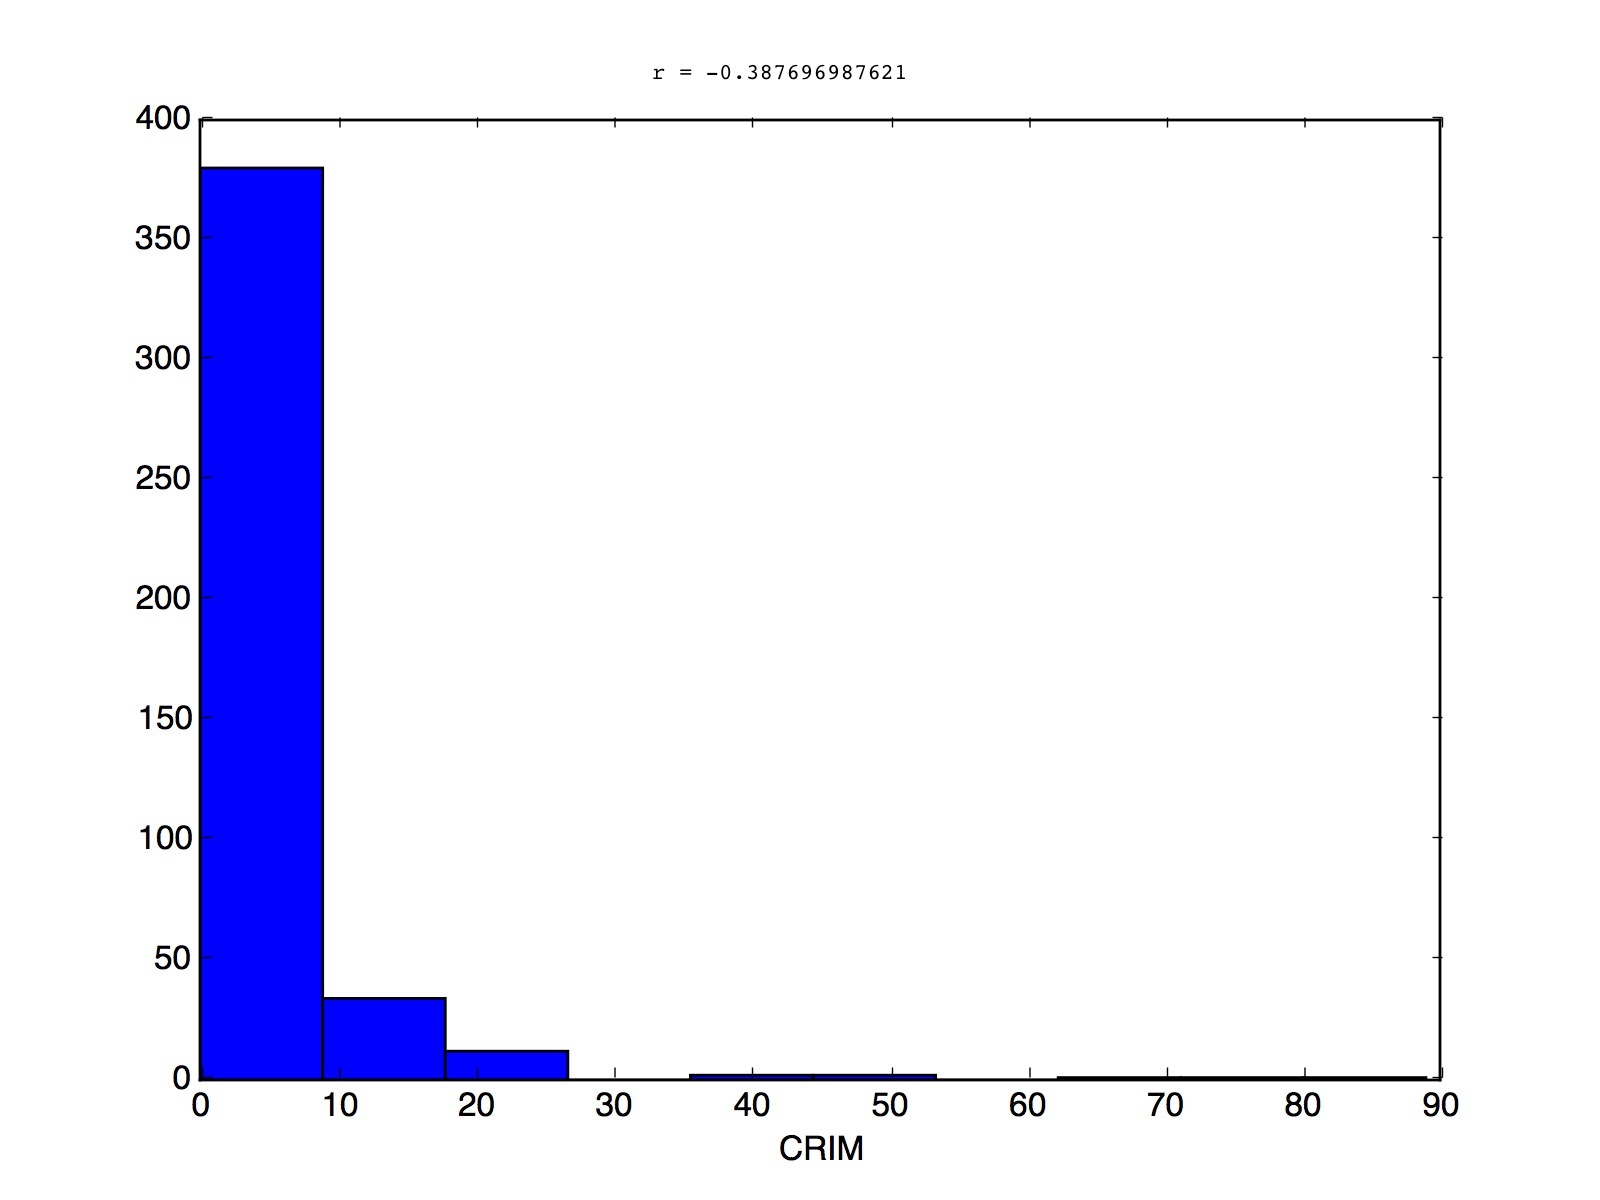
\includegraphics[scale=0.2]{hist_0}\\
			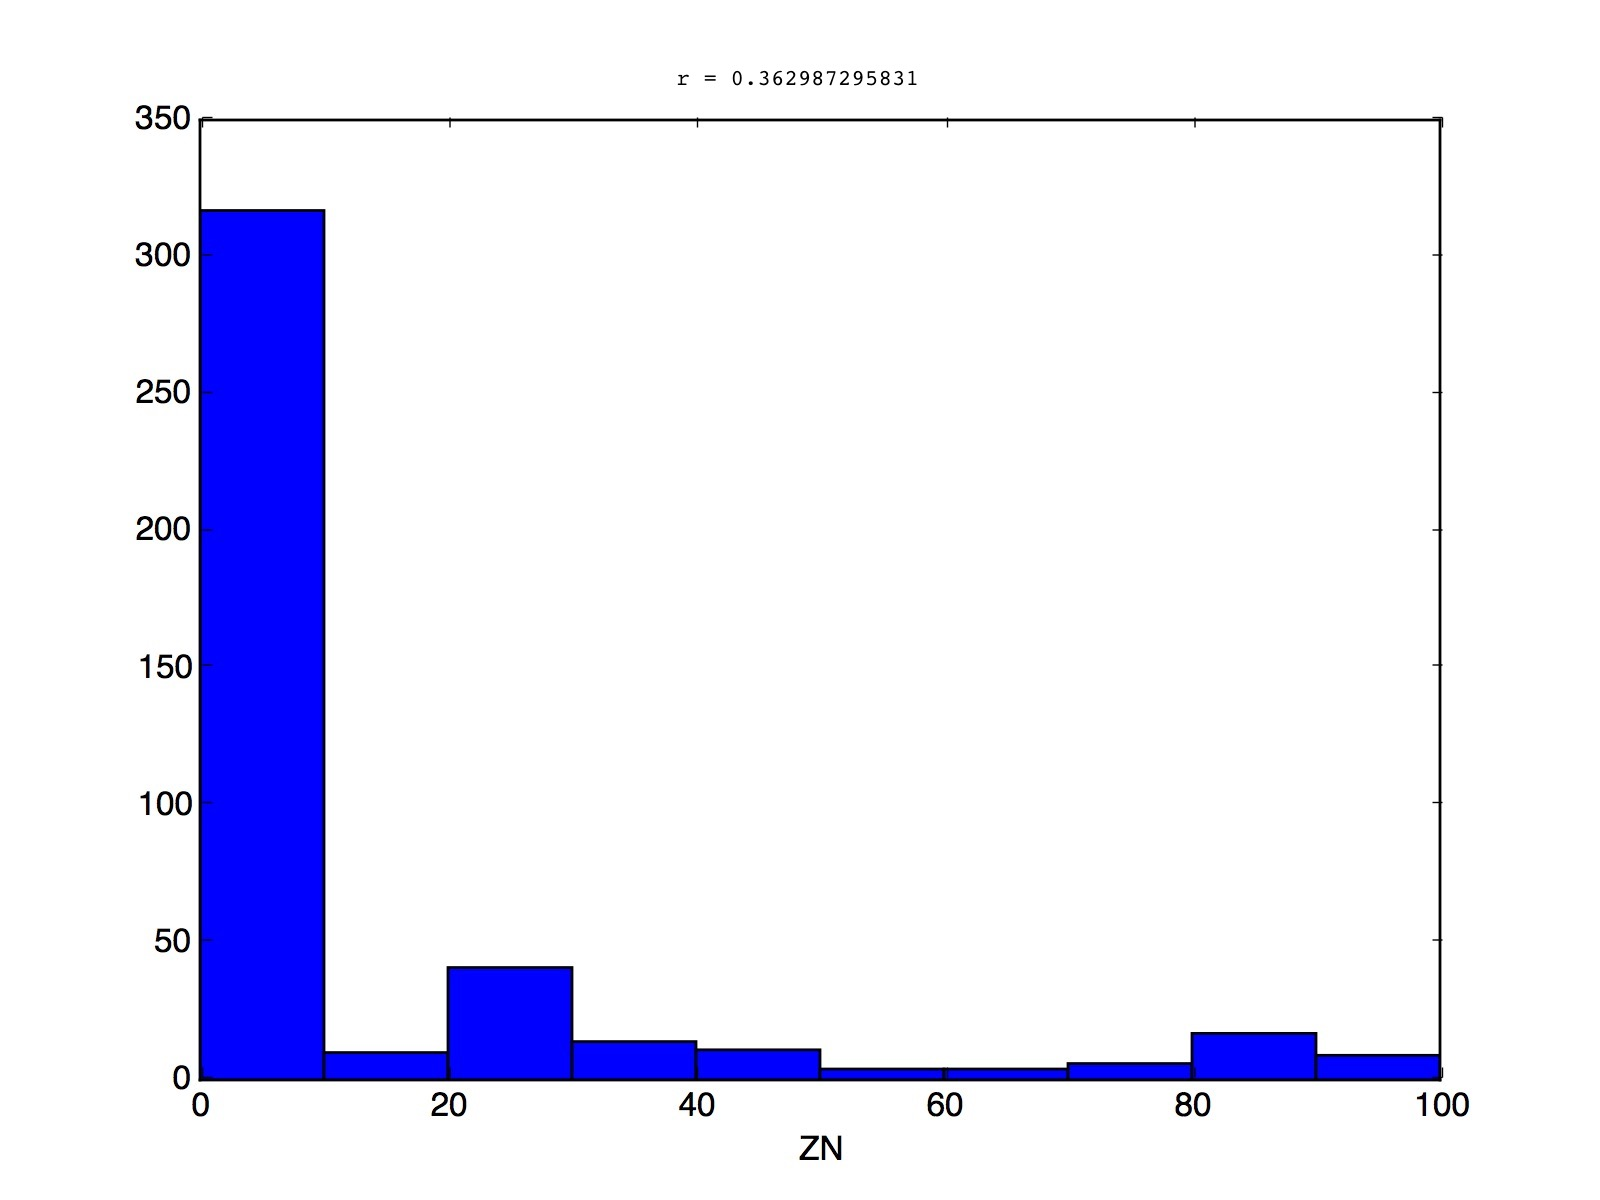
\includegraphics[scale=0.2]{hist_1}\\
			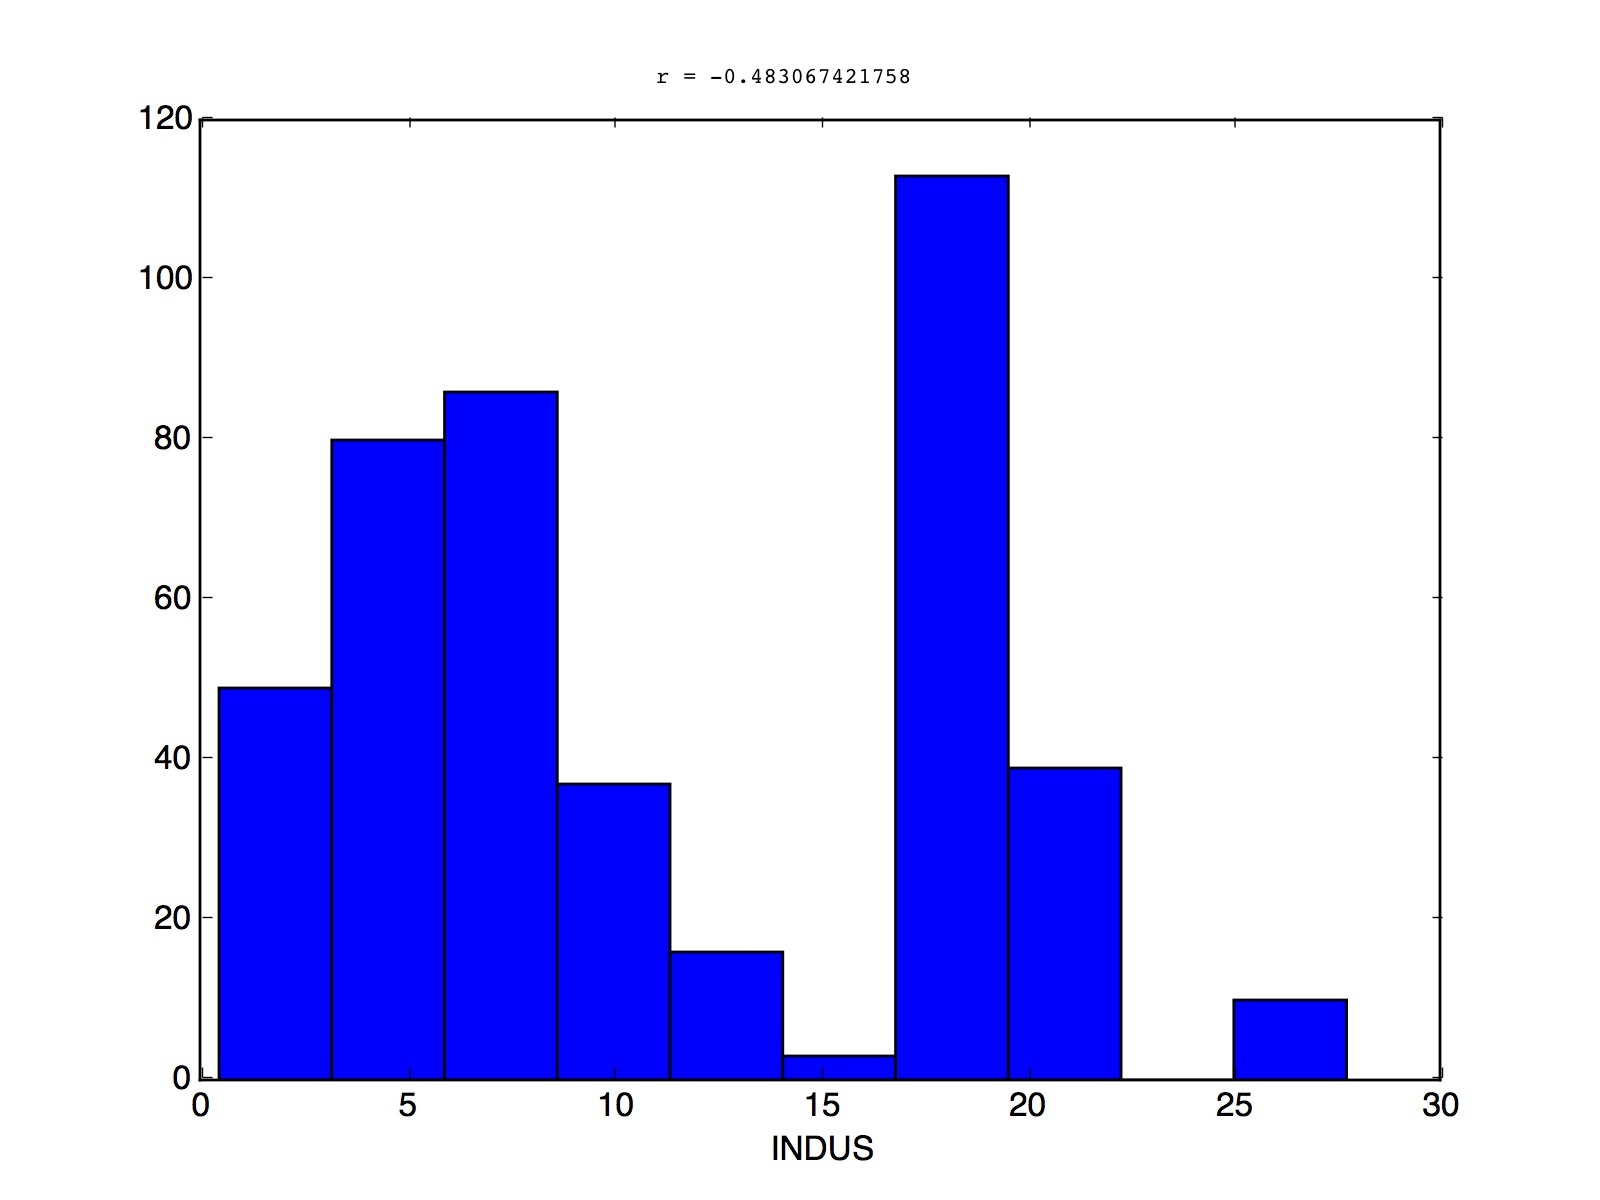
\includegraphics[scale=0.2]{hist_2}\\
			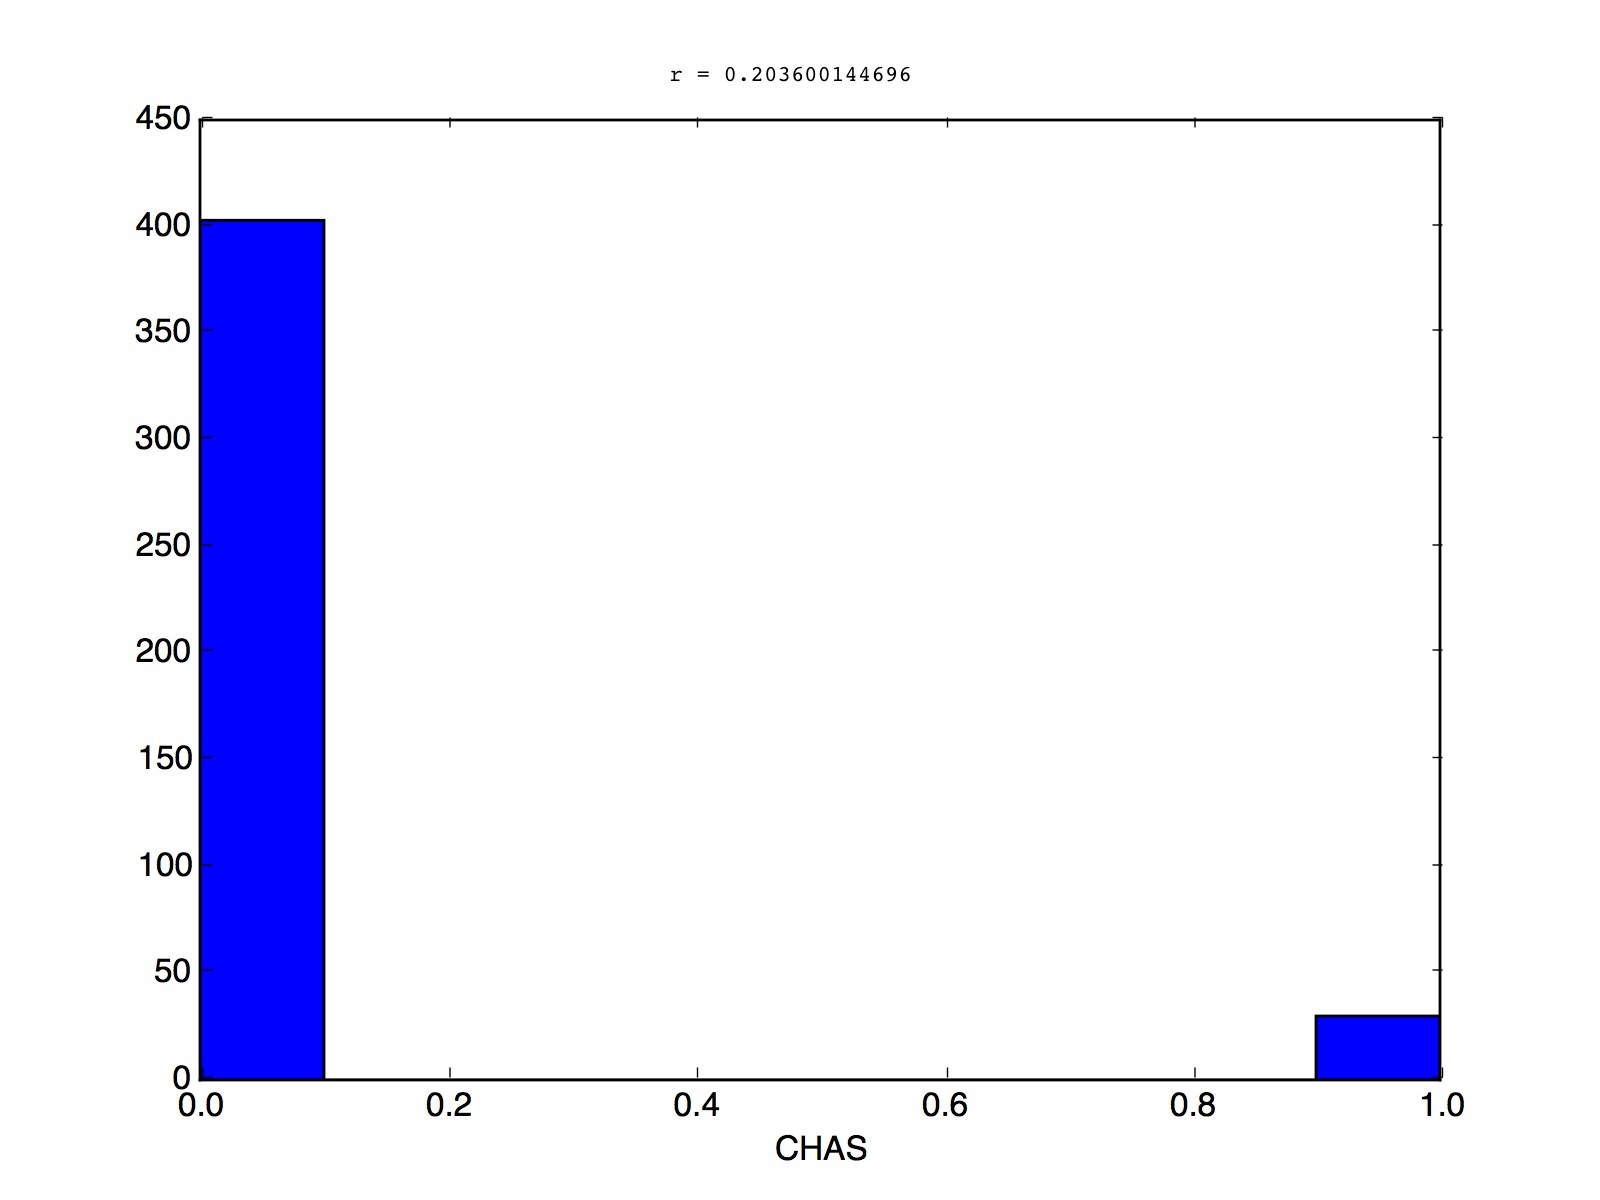
\includegraphics[scale=0.2]{hist_3}\\
			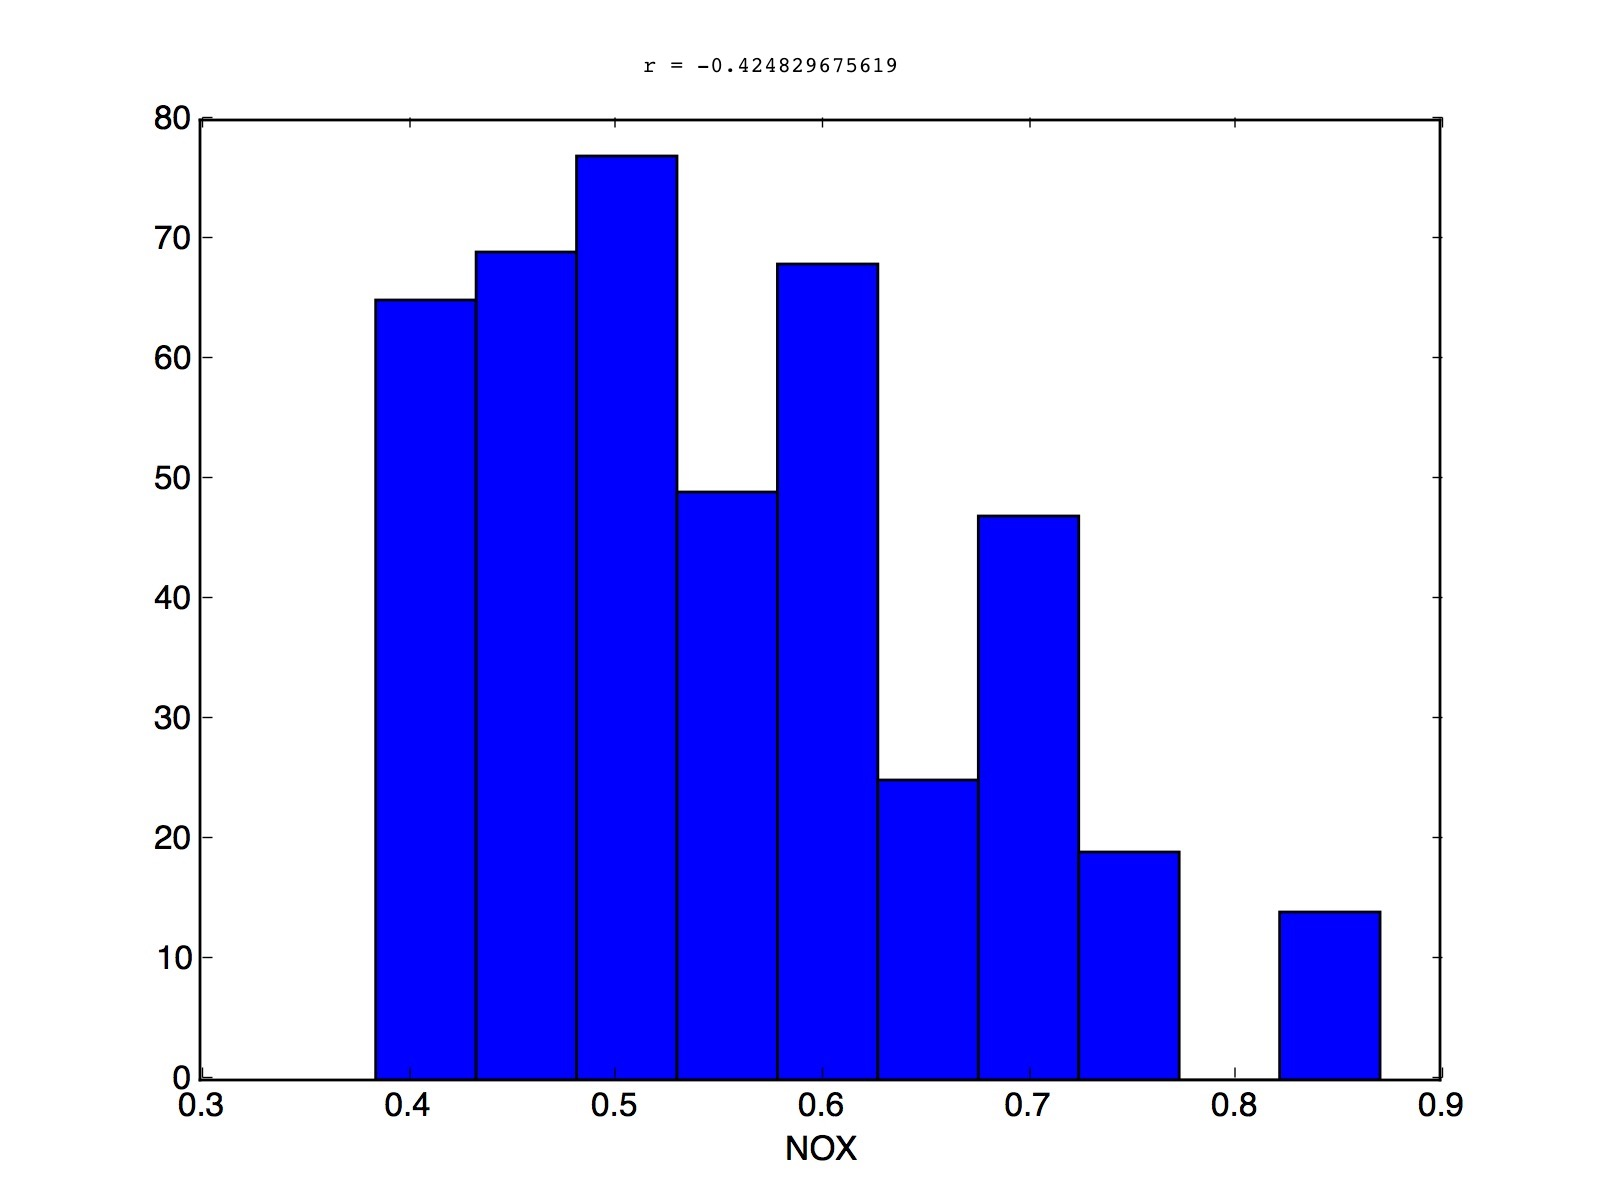
\includegraphics[scale=0.2]{hist_4}\\
			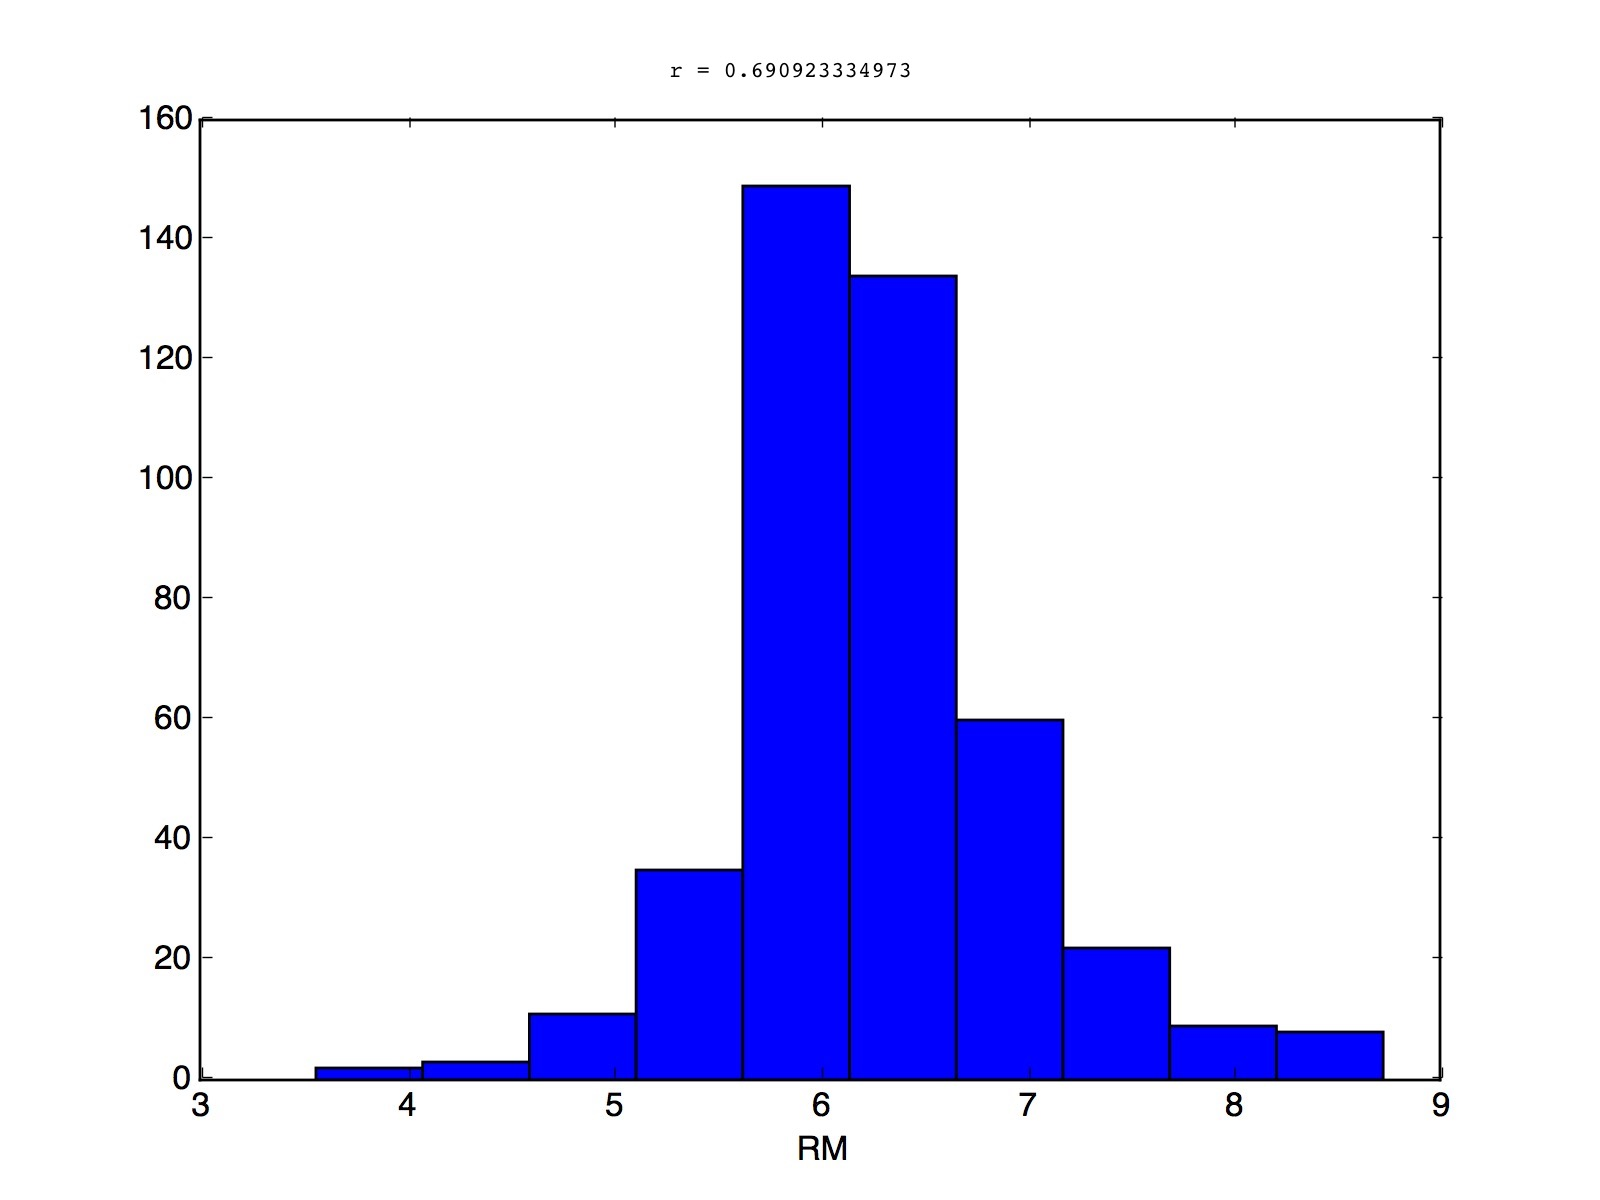
\includegraphics[scale=0.2]{hist_5}\\
			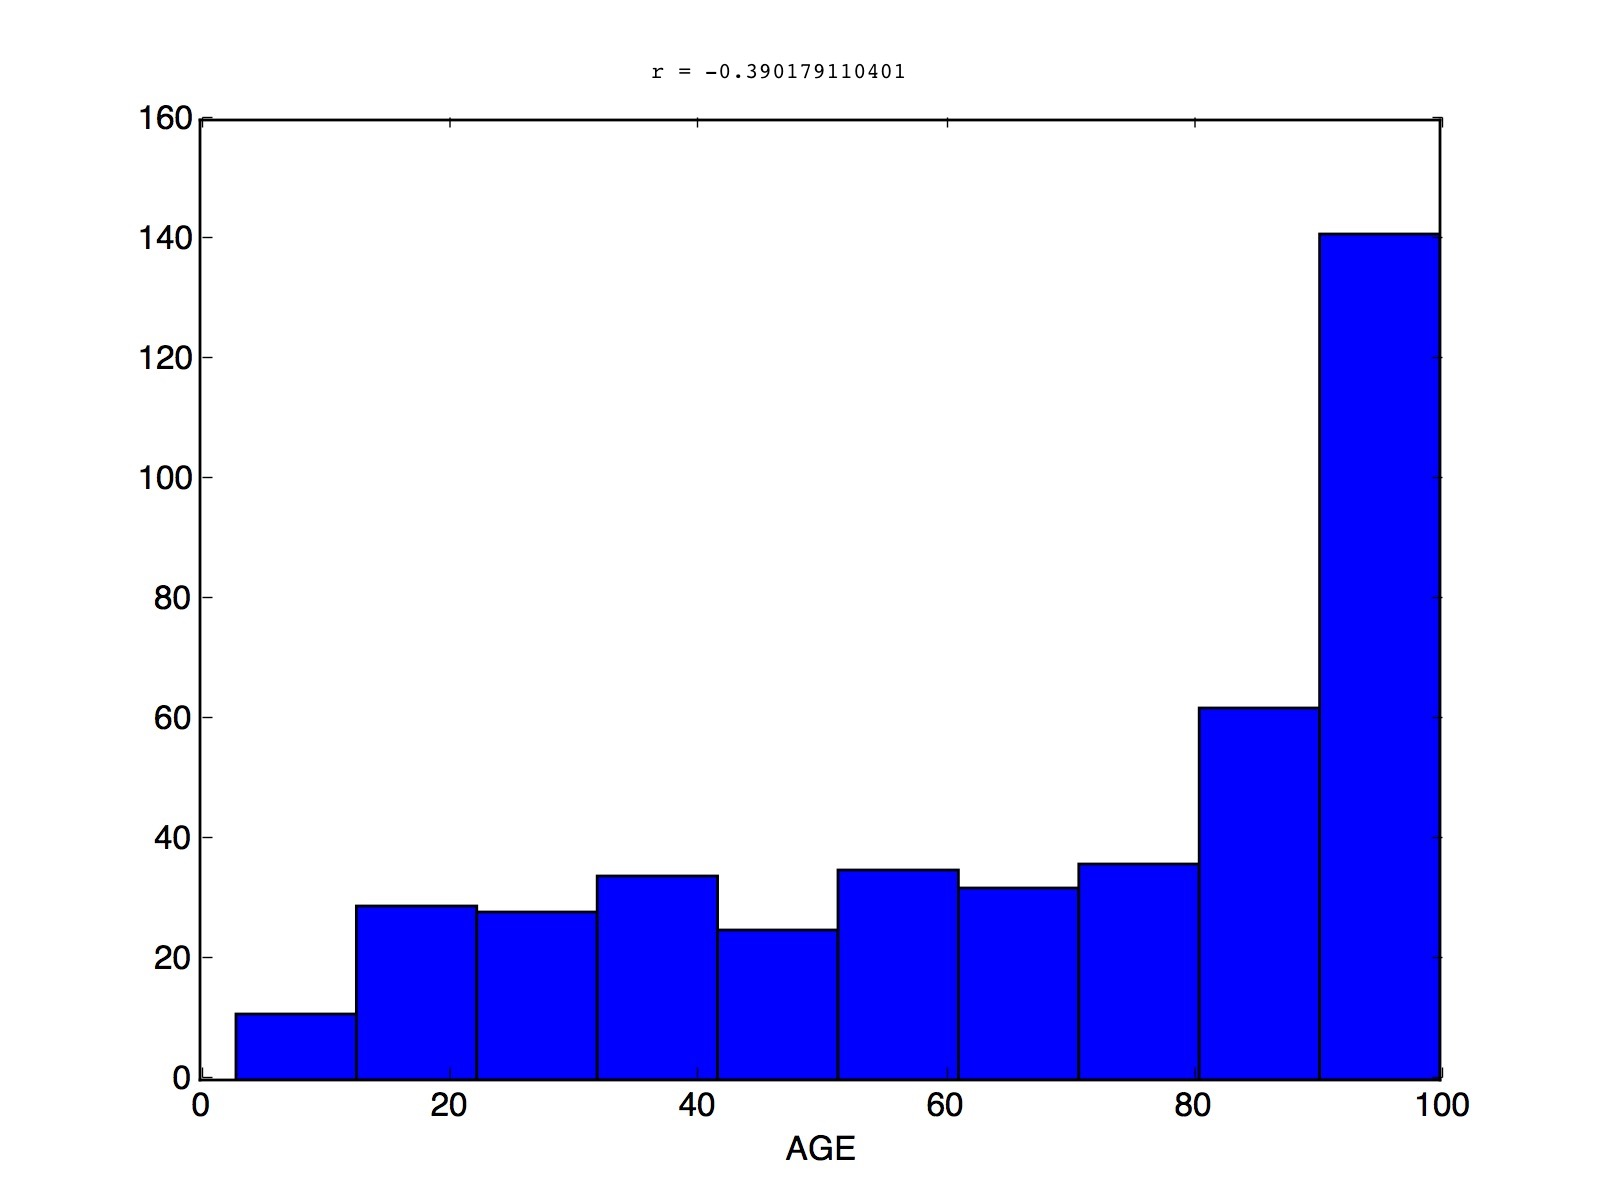
\includegraphics[scale=0.2]{hist_6}\\
			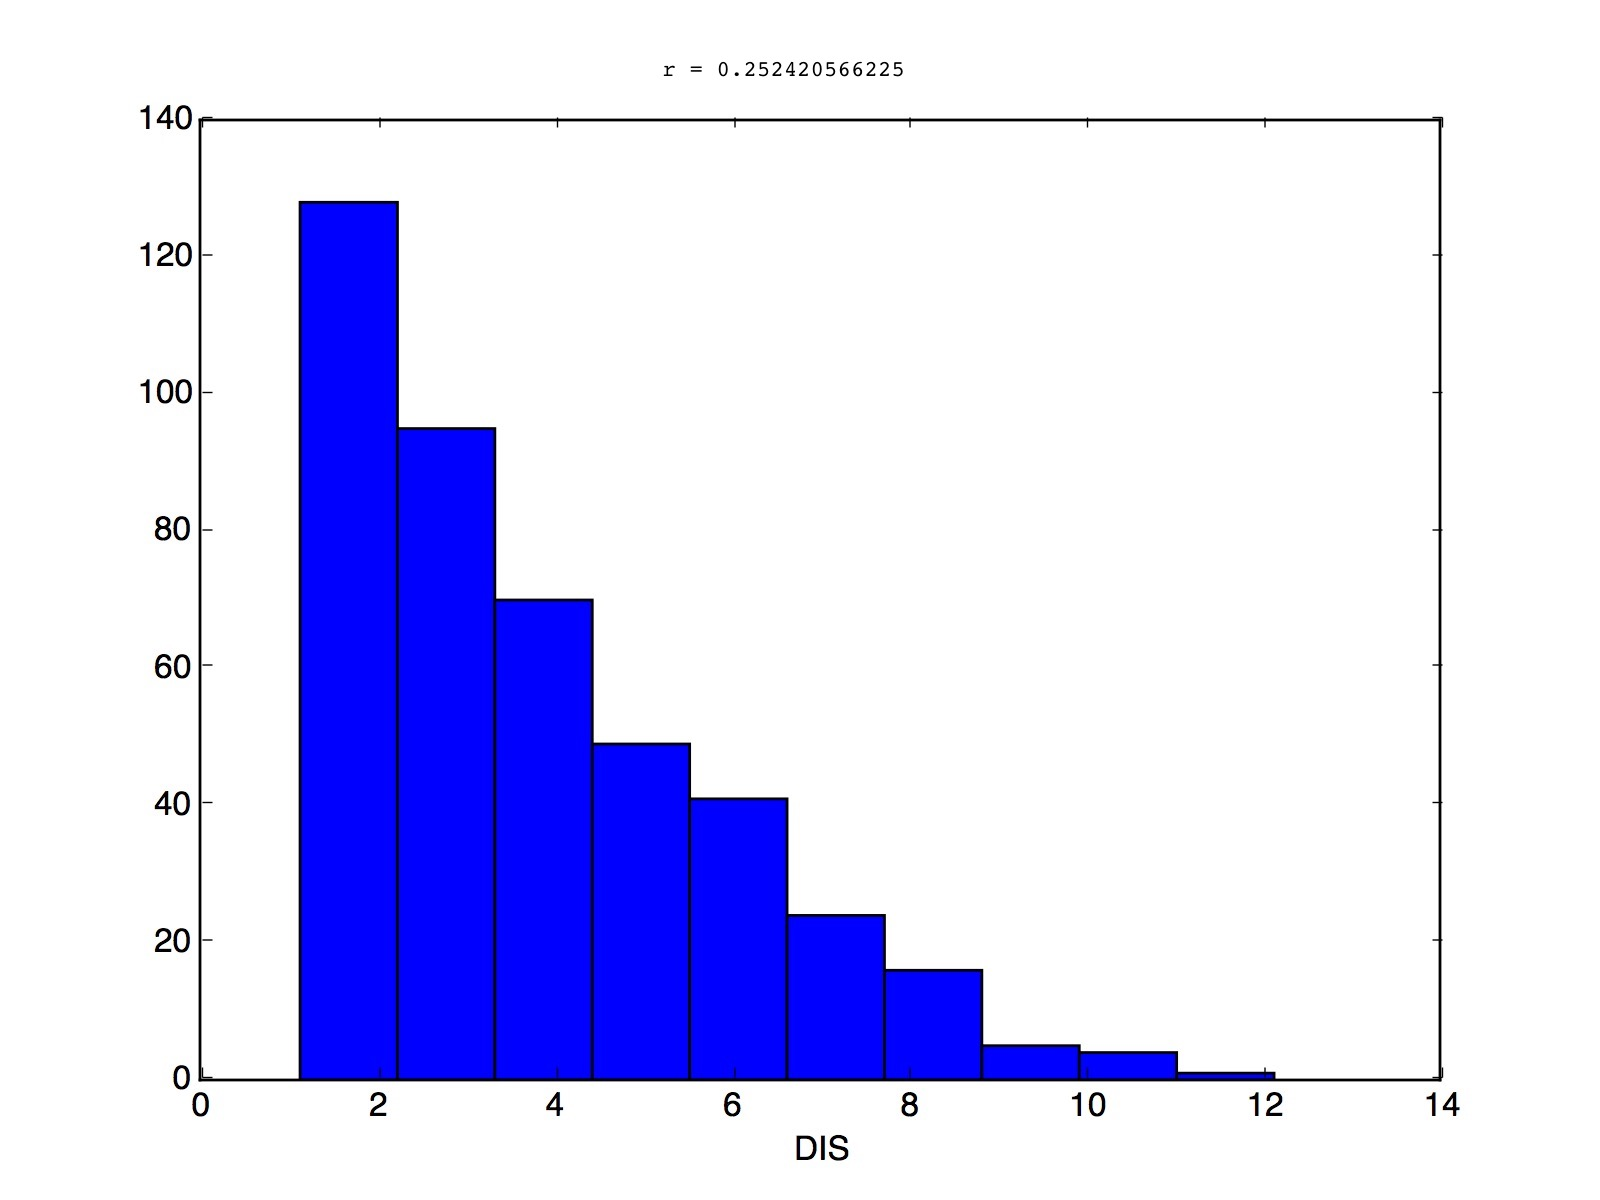
\includegraphics[scale=0.2]{hist_7}\\
			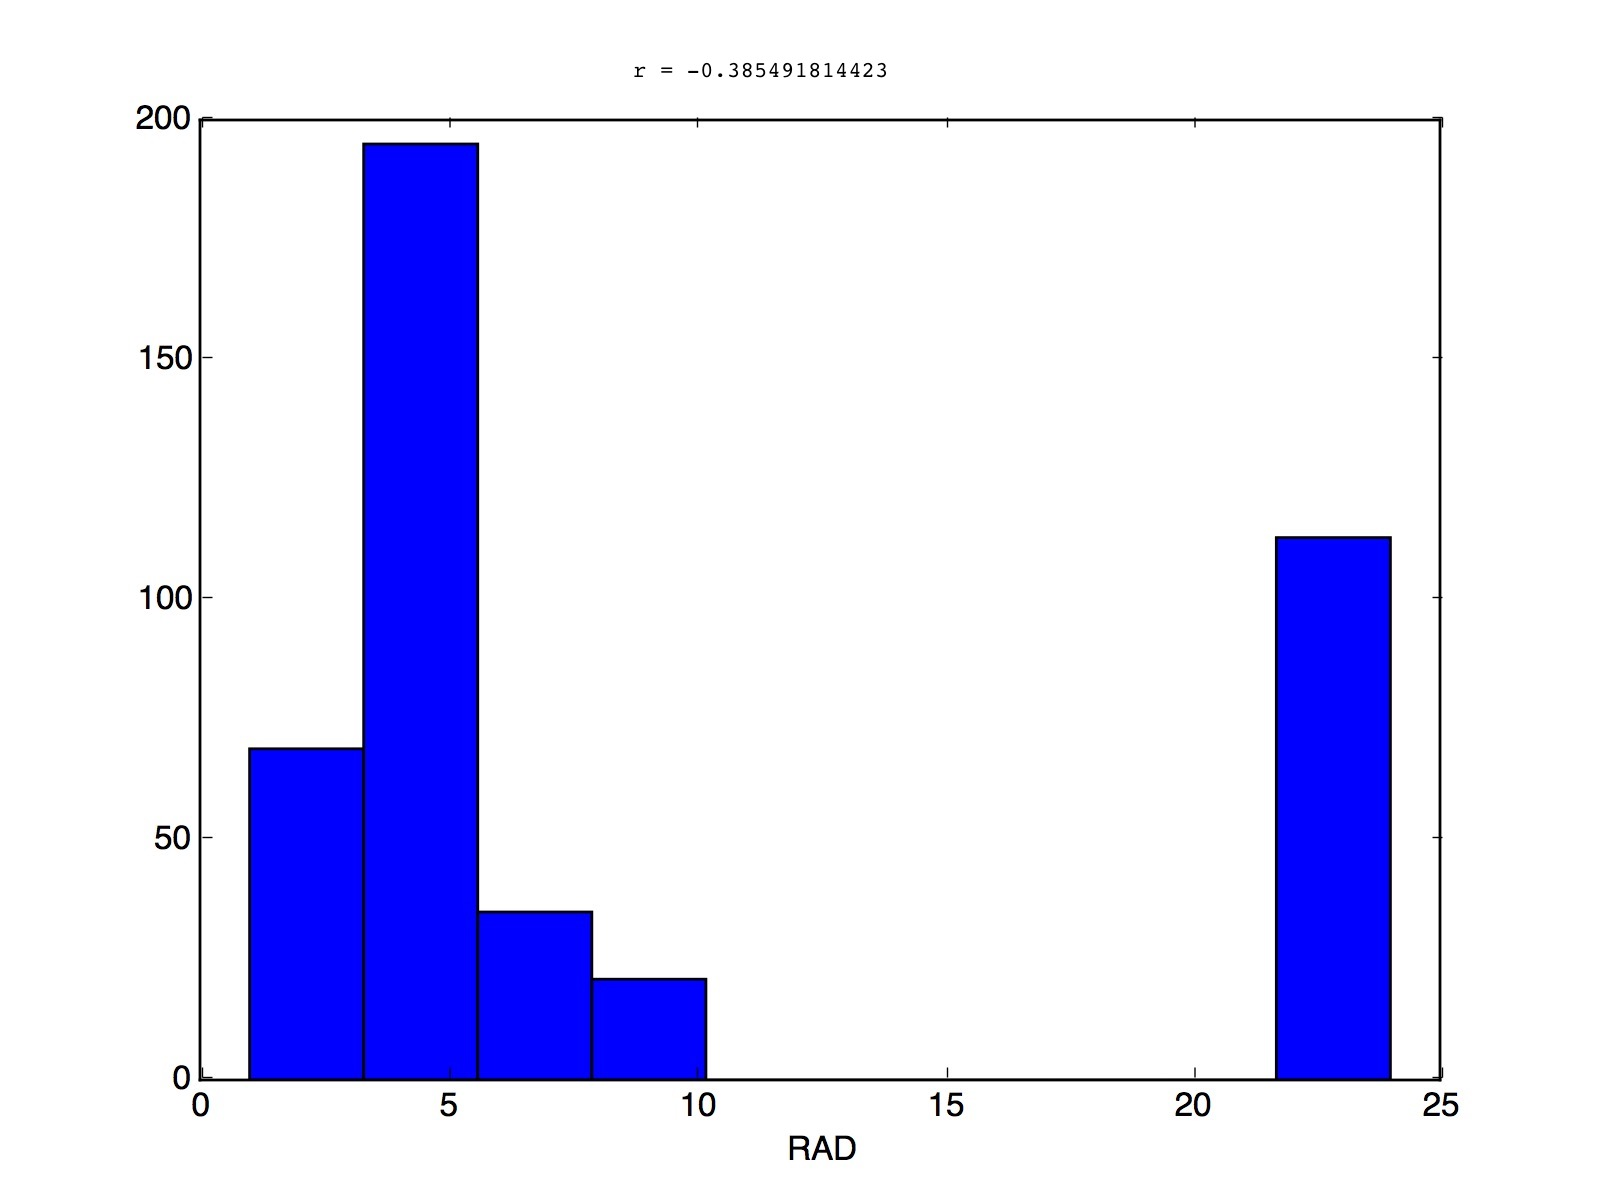
\includegraphics[scale=0.2]{hist_8}\\
			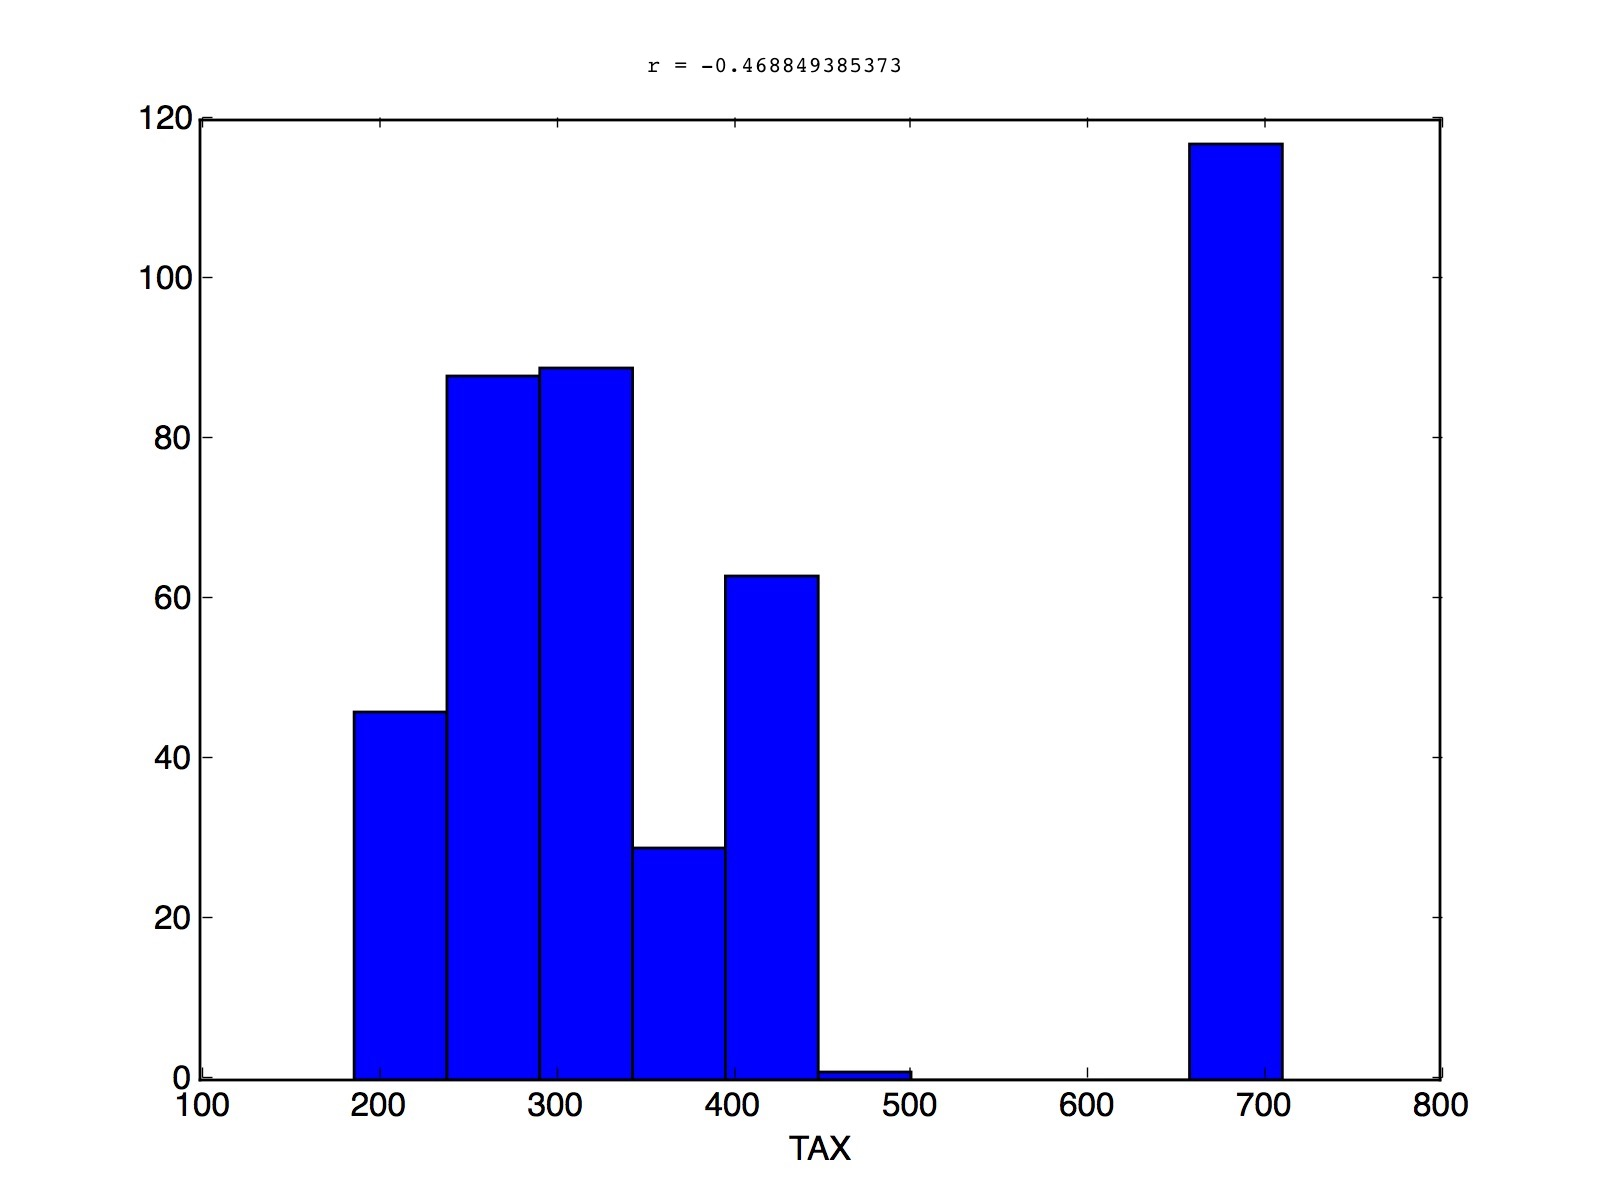
\includegraphics[scale=0.2]{hist_9}\\
			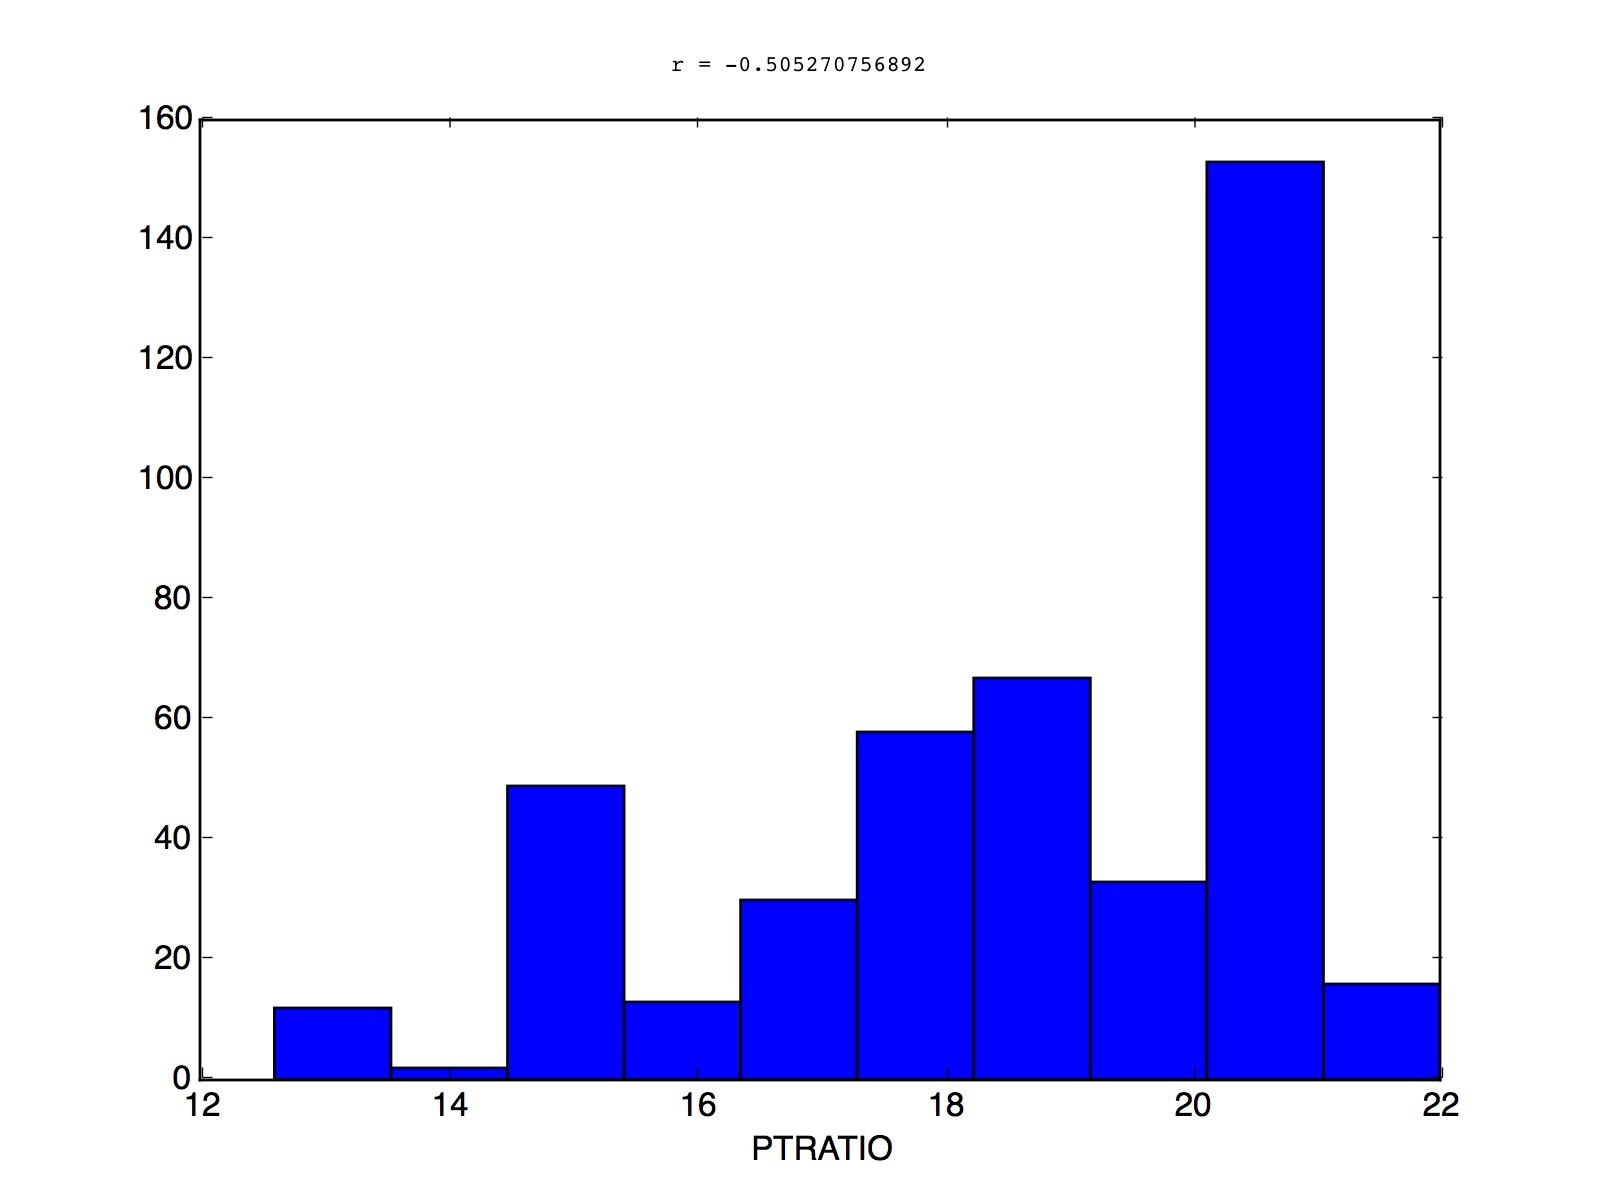
\includegraphics[scale=0.2]{hist_10}\\
			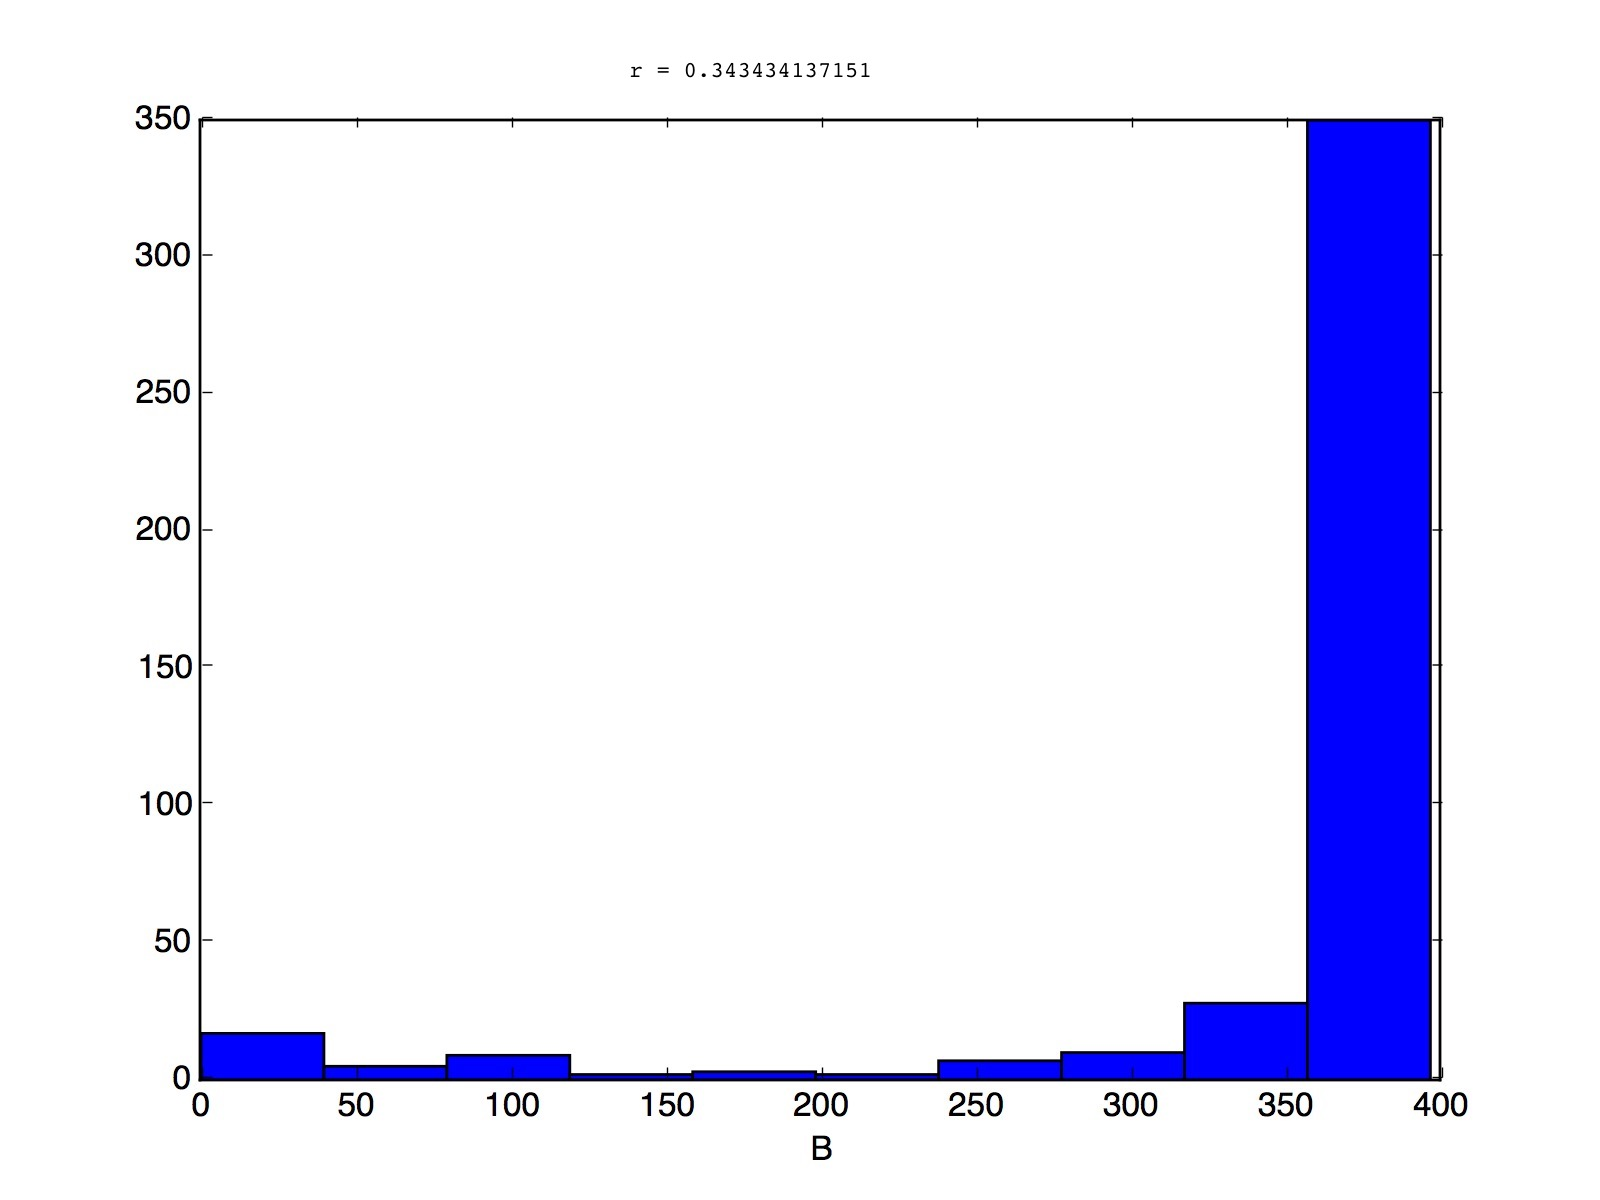
\includegraphics[scale=0.2]{hist_11}\\
			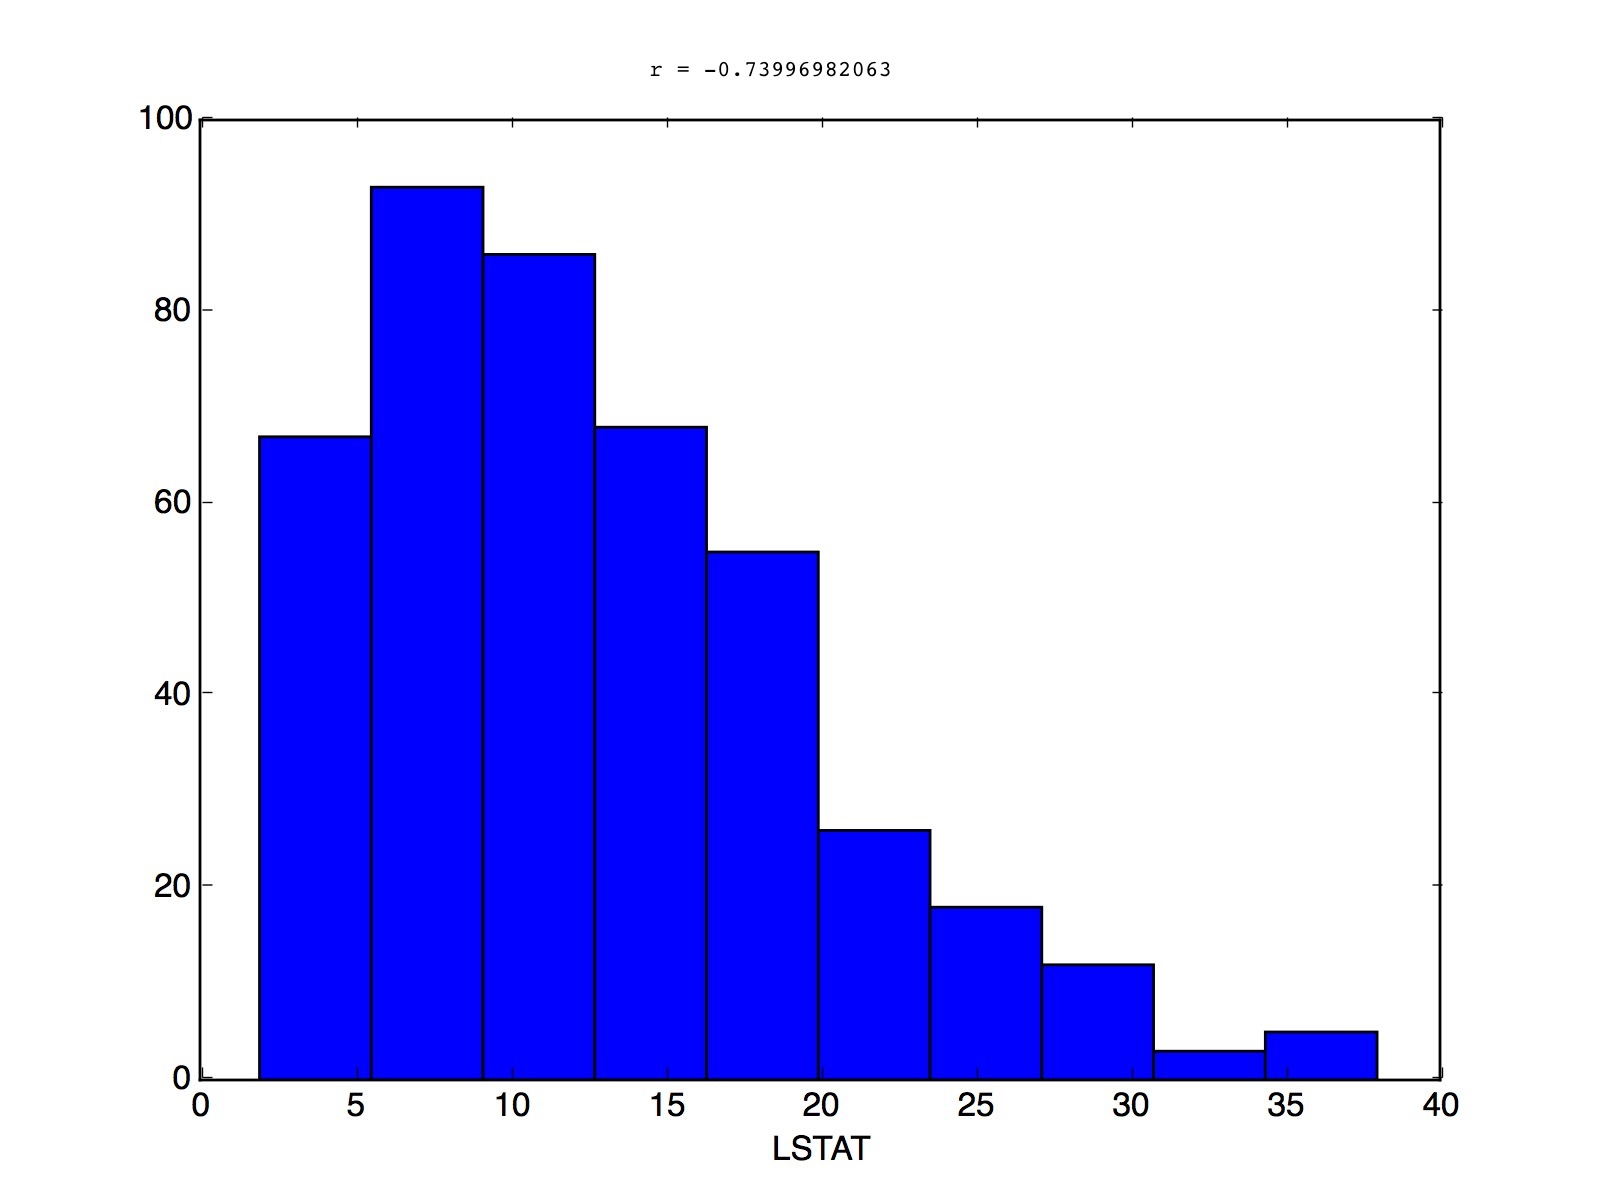
\includegraphics[scale=0.2]{hist_12}\\
		\end{center}

	\paragraph{Sol. 3.2}
		The after applying Linear Regression to the training set, we get the results

		\begin{center}
			\begin{tabular}{c|c}
				Test Data & MSE \\
				\hline
				test\_data & 28.4644 \\
				training\_data &20.9512 \\
				\hline
			\end{tabular}
		\end{center}

		%\newline
	
		After applying Ridge regression for different $\lambda$ we get the following results
		\begin{center}
		\begin{tabular}{c|c|c}
			\hline
			   	 $\lambda$ & Test Data    &     MSE \\
			\hline
			     0.01 & test\_data  & 28.4183 \\
			     0.01 & train\_data & 20.9501 \\
			     0.1  & test\_data  & 28.4217 \\
			     0.1  & train\_data & 20.9502 \\
			     1    & test\_data  & 28.4574 \\
			     1    & train\_data & 20.9539 \\
			\hline
		\end{tabular}
		\end{center}

		

		\begin{center}
		\begin{tabular}{c|c}
		\hline
		   $\lambda$ &     CVE \\
		\hline
		    0.001 & 9.99383 \\
		    0.01  & 9.99273 \\
		    0.02  & 9.9915  \\
		    0.1   & 9.98177 \\
		    0.1   & 9.98177 \\
		    1     & 9.8773  \\
		    2     & 9.77169 \\
		    3     & 9.67664 \\
		    4     & 9.59175 \\
		    5     & 9.51671 \\
		    6     & 9.45125 \\
		    7     & 9.39513 \\
		    8     & 9.34814 \\
		    9     & 9.31007 \\
		   10     & 9.28075 \\
		\hline
		\end{tabular}
		\end{center}

		As we see that the cross-validation error is minimum for $\lambda = 10$, therefore we choose $\lambda = 10$ for out MSE calculation.
		For \textbf{Test Data set we get MSE = 28.98456207} and for \textbf{Training Data set we get MSE = 21.28681485}.
		
		\paragraph{Sol. 3.3.a}
		First, we will calculate the Pearson's Coefficient for each attribute with target values and we get 
		\begin{center}
		\begin{tabular}{c | c}
			\hline
			 Feature   &   abs(r) \\
			\hline
			 CRIM      & 0.387697 \\
			 ZN        & 0.362987 \\
			 INDUS     & 0.483067 \\
			 CHAS      & 0.2036   \\
			 NOX       & 0.42483  \\
			 RM        & 0.690923 \\
			 AGE       & 0.390179 \\
			 DIS       & 0.252421 \\
			 RAD       & 0.385492 \\
			 TAX       & 0.468849 \\
			 PTRATIO   & 0.505271 \\
			 B         & 0.343434 \\
			 LSTAT     & 0.73997  \\
			\hline
			\end{tabular}
		\end{center}

		We see that the attributes with highest Pearson's Coefficients are INDUS, PTRATIO, RM, LSTAT.\\

		Now, applying \textbf{Linear Regression}
	    \begin{center}
	    \begin{tabular}{c | c}
	        \hline
	        Test Data & MSE \\
	        \hline
	        test\_data & 31.4962 \\
	        train\_data & 26.4066
	    \end{tabular}
	    \end{center}

	    Now, applying Ridge Regression for different $\lambda$ we get

	    \begin{center}
	    \begin{tabular}{c|c|c}
			\hline
			   $\lambda$ & Test Data    &     MSE \\
			\hline
			     0.01 & test\_data  & 31.496  \\
			     0.01 & train\_data & 26.4066 \\
			     0.1  & test\_data  & 31.4944 \\
			     0.1  & train\_data & 26.4066 \\
			     1    & test\_data  & 31.4806 \\
			     1    & train\_data & 26.4094 \\
			\hline
		\end{tabular}
	    \end{center}

	    For K-Fold Ridge Regression we get the following values of CVE

	    \begin{center}
	    \begin{tabular}{c | c}
			\hline
			   $\lambda$ &    CVE \\
			\hline
			    0.001 & 8.3003 \\
			    0.01  & 8.2992 \\
			    0.1   & 8.2885 \\
			    1     & 8.1855 \\
			    2     & 8.0791 \\
			    3     & 7.9811 \\
			    4     & 7.8915 \\
			    5     & 7.8099 \\
			    6     & 7.7363 \\
			    7     & 7.67   \\
			    8     & 7.6125 \\
			    9     & 7.562  \\
			   10     & 7.5189 \\
			\hline
			\end{tabular}
	    \end{center}

	  	Choosing $\lambda = 10$, we get the MSE as 
	  	
		\begin{center}
	    \begin{tabular}{c|c|c}
			\hline
			   $\lambda$ & Test Data    &     MSE \\
			\hline
			     10 & test\_data  & 31.5937  \\
			     10 & train\_data & 26.6775 \\
			\hline
		\end{tabular}
	    \end{center}

	\paragraph{Sol. 3.3.b}
	    From the previous exercise we know that the feature with the highest correlation coefficient with the target is LSTAT.

	    Now, calculating residue and correlation coefficient of the rest of the attributes with the residue we get

	    \begin{center}
	    \begin{tabular}{c|c}
			\hline
			 Feature & abs(r(residue, attr\_vals)  \\
			\hline
			 CRIM    & 0.426588158091 \\
			 ZN      & 0.398133315751 \\
			 INDUS   & 0.537842703653 \\
			 CHAS    & 0.175073939283 \\
			 NOX     & 0.491958859016 \\
			 RM      & 0.702473672384 \\
			 AGE     & 0.469369575525 \\
			 DIS     & 0.331853691887 \\
			 RAD     & 0.436013562838 \\
			 TAX     & 0.514184631153 \\
			 PTRATIO & 0.496710217811 \\
			 B       & 0.374589793897 \\
			\hline
			\end{tabular}
	    \end{center}

	    We get RM as the next feature with highest correlation coefficient. \\

	    After updating the residue, we get the correlation coeff. as

	    \begin{center}
	    \begin{tabular}{c|c}
			\hline
			 Feature & abs(r(residue, attr\_vals)  \\
			\hline
			 CRIM    & 0.129554112358  \\
			 ZN      & 0.0461901567406 \\
			 INDUS   & 0.0561934824677 \\
			 CHAS    & 0.249301273706  \\
			 NOX     & 0.0109129511978 \\
			 AGE     & 0.0159396362859 \\
			 DIS     & 0.134713549718  \\
			 RAD     & 0.087477994304  \\
			 TAX     & 0.13681944445   \\
			 PTRATIO & 0.297604744231  \\
			 B       & 0.156620202695  \\
			\hline
			\end{tabular}
	    \end{center}

	    We get PTRATIO as the next feature with highest correlation coefficient. \\

	    Again,
	    \begin{center}
	    \begin{tabular}{c|c}
			\hline
			 Feature & abs(r(residue, attr\_vals)  \\
			\hline
			 CRIM    & 0.0889293951571  \\
			 ZN      & 0.0323063735902  \\
			 INDUS   & 0.00214795182009 \\
			 CHAS    & 0.2195949638     \\
			 NOX     & 0.0198942311859  \\
			 AGE     & 0.0435891823287  \\
			 DIS     & 0.170389023828   \\
			 RAD     & 0.0210281033187  \\
			 TAX     & 0.0440426778355  \\
			 B       & 0.144133379832   \\
			\hline
		\end{tabular}
	    \end{center}

	  	Finally, we select the feature CHAS.\\

	  	So, finally our selected features (in-order) are LSTAT, RM, PTRATIO, CHAS. \\

	  	Now, calculating MSE from previously fitted data, we get

	  	\begin{center}
	  	\begin{tabular}{c|c}
			\hline
			 Input Data   &     MSE \\
			\hline
			 test\_data    & 34.5988 \\
			 train\_data   & 25.106  \\
			\hline
			\end{tabular}
	  	\end{center}

	  	\textbf{Brute Force}: The best combination is B, RM, LSTAT, PTRATIO with $MSE = 30.09226$ with test data set.

	  \paragraph{Sol. 3.4}
	  	The result after calculating the MSE using Linear Regression with the augmented data is

	  	\begin{center}
	  	\begin{tabular}{c|c}
			\hline
			 Input Data   &     MSE \\
			\hline
			 test\_data    & 14.5553 \\
			 train\_data   & 5.05978 \\
			\hline
			\end{tabular}
	  	\end{center}

\end{document}